\documentclass[tikz,border=10pt]{standalone}
\usepackage{amsmath}
\usetikzlibrary{calc}
\begin{document}
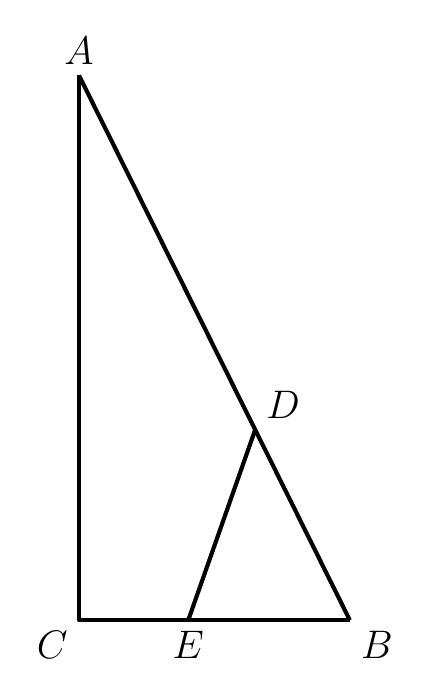
\begin{tikzpicture}[line join=round, line width=1.5pt]
\coordinate (A) at (-1.550,3.459);
\coordinate (B) at (1.890,-3.459);
\coordinate (C) at (-1.550,-3.459);
\coordinate (D) at (0.688,-1.041);



\coordinate (E) at (-0.162,-3.459);


\draw (A) -- (C) -- (B);
\draw (A) -- (D) -- (B);


\draw (D) -- (E);


\node[above] at (A) {\fontsize{14.5}{17.4}\selectfont $A$};
\node[below right] at (B) {\fontsize{14.5}{17.4}\selectfont $B$};
\node[below left] at (C) {\fontsize{14.5}{17.4}\selectfont $C$};
\node[above right] at (D) {\fontsize{14.5}{17.4}\selectfont $D$};
\node[below] at (E) {\fontsize{14.5}{17.4}\selectfont $E$};
\end{tikzpicture}
\end{document}